\section{Specifications}
\newcounter{rulei}[subsection]
\newcommand{\rcnii}{\stepcounter{rulei}\arabic{section}.\arabic{subsection}.\arabic{rulei}}
\renewcommand{\labelenumi}{\rcnii}

\subsection{Arena}
\begin{enumerate}
\item The match arena is a 8m x 8m square.  The tolerance of the two arena dimensions is $\pm0.5m$.
\item The floor of the arena is made of white plastic coated hardboard.
\item The hardboard is joined with white Gaffer tape.
\item The arena walls are $600\pm30mm$ high and are made of the same material as the arena floor.
\item The wall-to-floor join is bridged in white Gaffer tape.
\end{enumerate}

\subsection{Tokens}
\label{tokens}

\begin {enumerate} 
\item Tokens are cubes of side 45$\pm5mm$.
\item Tokens weigh 40$\pm10g$
\end {enumerate}

\subsection{Zones}
\begin {enumerate}
\item The arena contains 4 zones.  Each zone is located at a corner of the arena.  See figure~\ref{fig:arena}.
\item A zone is a 1.5m x 1.5m square.  The tolerance of the zone dimensions is $\pm50mm$.
\item The zone is bounded by the zone border.  The zone border is $135\pm5mm$ (3 tokens) in width.
\item Each zone has an associated colour.  The zone border is this colour.
\item The zone is split into two areas.  The main zone and the bonus zone.  See figure~\ref{fig:zone}.
\item The bonus zone and main zone are divided by a white barrier of square cross-section.  The height of this barrier is $45\pm5mm$ (token height).  Figure~\ref{fig:zone} shows this barrier.
\end {enumerate}

\begin{figure}
\begin{center}
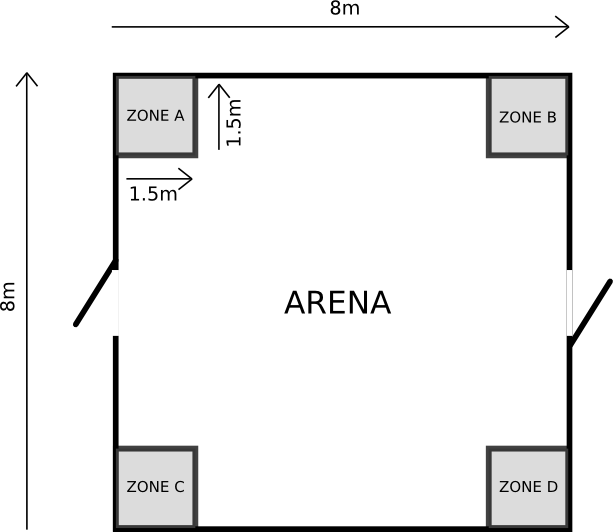
\includegraphics[keepaspectratio, width=\textwidth]{./images/arenadim.png}
\caption{\label{fig:arena}Zone Dimensions}
\end{center}
\end{figure}

\begin{figure}
\begin{center}
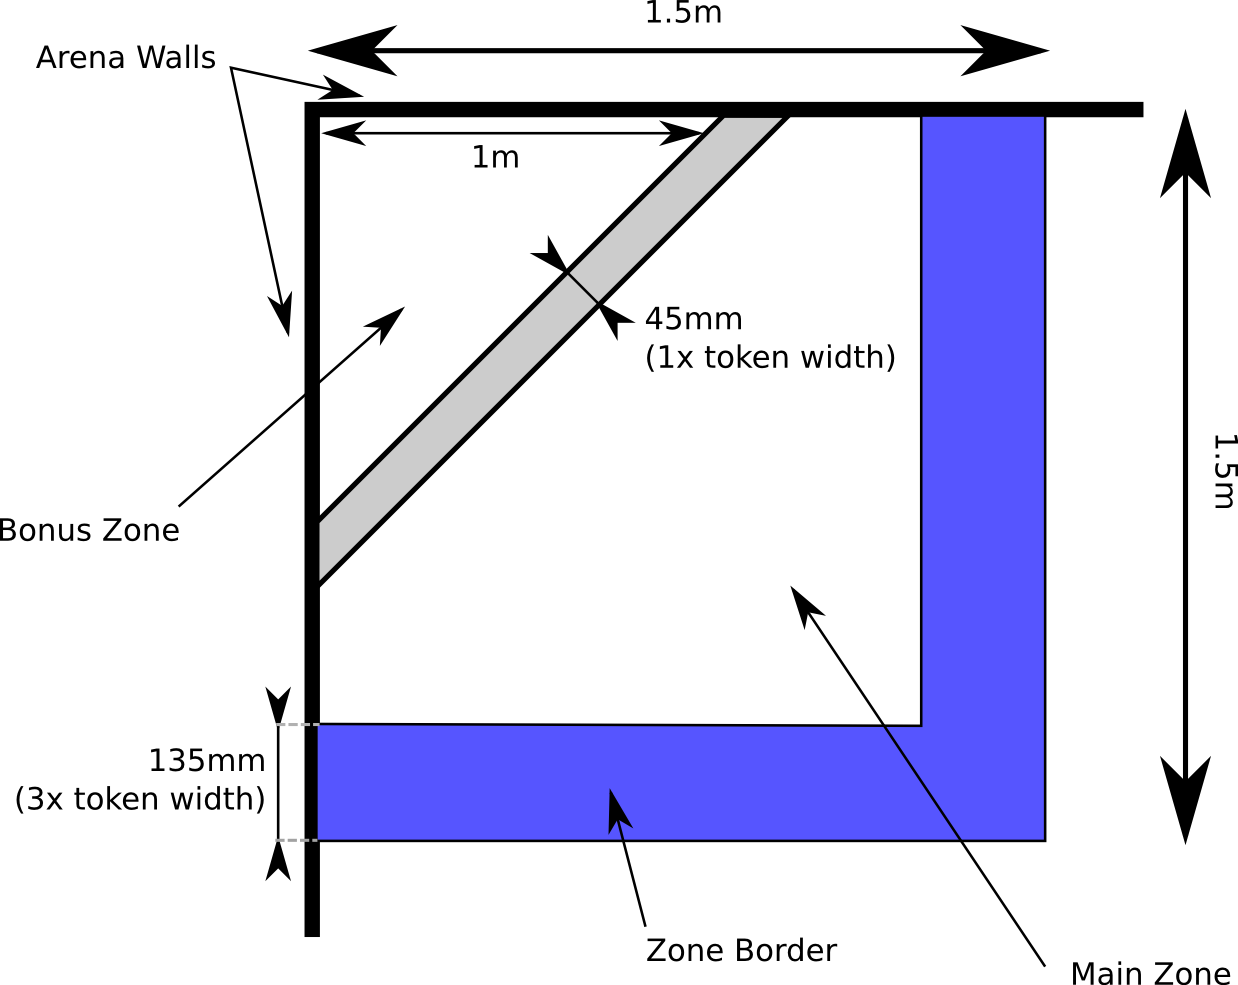
\includegraphics[keepaspectratio, scale =1]{./images/zone.png}
\caption{\label{fig:zone}Zone Dimensions}
\end{center}
\end{figure}

\subsection{Obstacles}
\begin{enumerate}
\item The arena will contain between 0 and 6 obstacles.
\item An obstacle is entirely black.
\item An obstacle has the shape described by figure~\ref{fig:obstacle}.
\end{enumerate}

\begin{figure}
\begin{center}
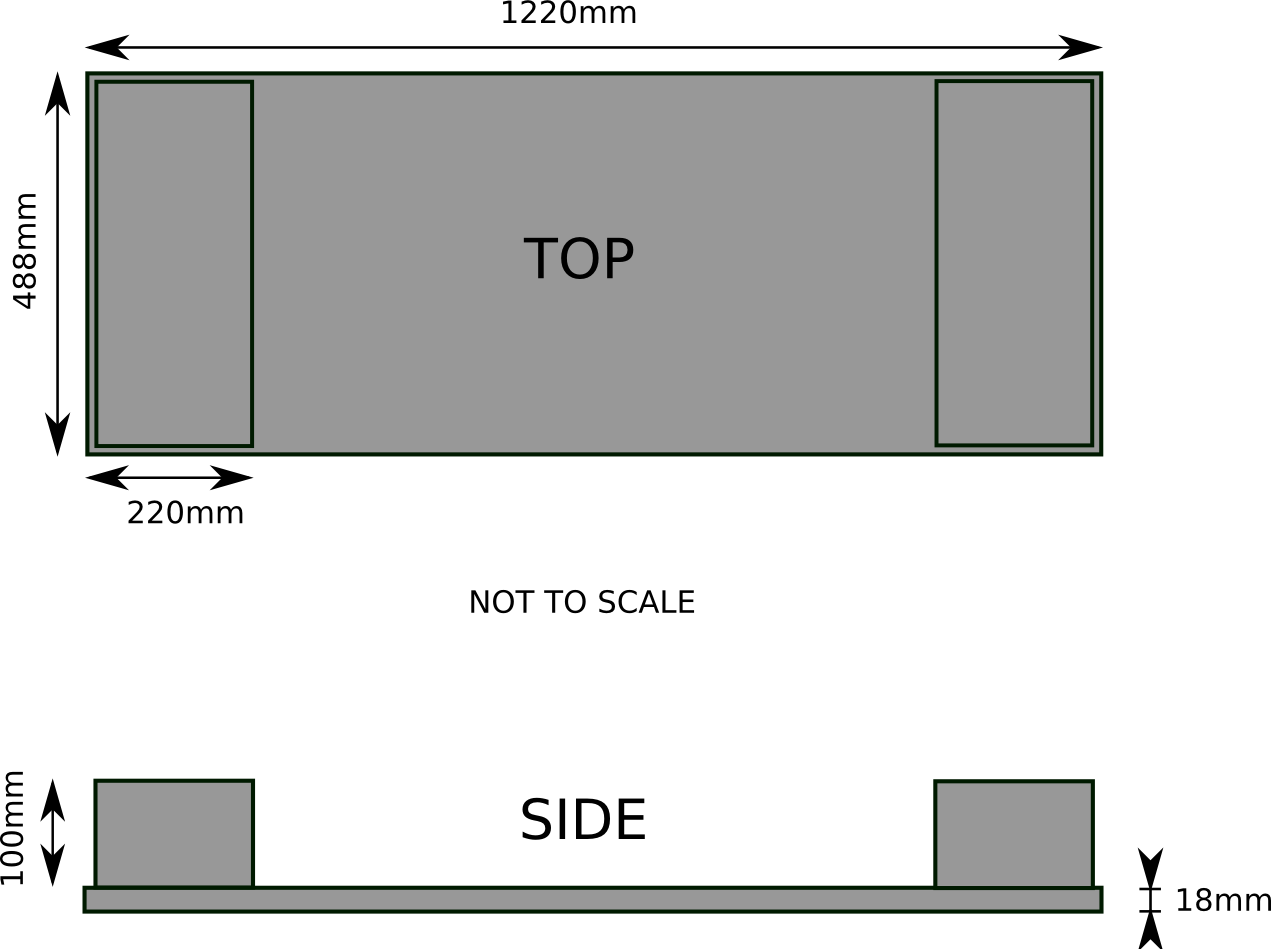
\includegraphics[keepaspectratio, scale =1]{./images/obstacle.png}
\caption{\label{fig:obstacle}Obstacle Dimensions}
\end{center}
\end{figure}

\subsection{Robot Flags}
\label{sec:flags}
All robots must have a flagpole so that two flags can be mounted upon it:
\begin{description}
\item[Team Flag] The team flag is to be designed and created by the team.  It is optional and recommended.  The team flag is to allow the robot to be easily identifiable.  This flag must be mounted between 700mm and 900mm off the ground.  It must not extend more than 200mm from the flagpole.

The team flag must not sag below 700mm above the ground.
\item[Match Flag] The match flag is to be supplied by Student Robotics at the start of every match.  The match flag will slot over the top 100mm of the flagpole.  The top 100mm of the flagpole must have an external diameter of $5\pm1$mm so that the match flag can slot over it.  The match flags have an end-cap so that they will not slide down the flagpole.
\end{description}

It is recommended that the flagpole be easily removable so that the robot can easily be placed within a box to check the size limit.  A diagram of the flagpole arrangement can be found in figure~\ref{fig:flag}.

\begin{figure}
\begin{center}
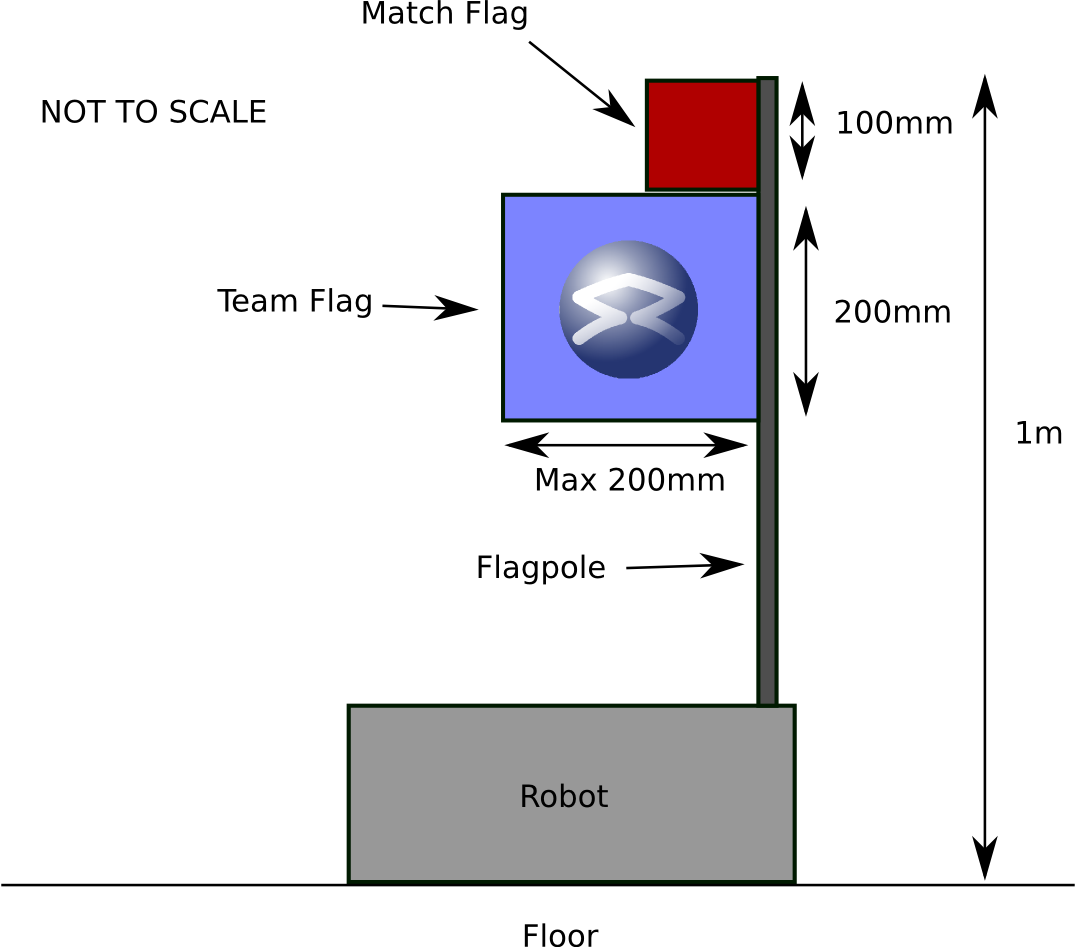
\includegraphics[keepaspectratio, scale =1]{./images/flag.png}
\caption{\label{fig:flag}Flagpole Dimensions}
\end{center}
\end{figure}
